%
% ---------- header -----------------------------------------------------------
%
% project       kaneton
%
% license       kaneton
%
% file          /home/mycure/kaneton/view/book/kaneton/kaneton.tex
%
% created       julien quintard   [mon may 14 19:56:45 2007]
% updated       julien quintard   [sun dec 16 17:23:52 2007]
%

%
% ---------- setup ------------------------------------------------------------
%

%
% path
%

\def\path{../..}

%
% template
%

%
% ---------- header -----------------------------------------------------------
%
% project       kaneton
%
% license       kaneton
%
% file          /home/mycure/kaneton/view/template/book.tex
%
% created       julien quintard   [wed may 16 18:16:50 2007]
% updated       julien quintard   [sun jun  3 12:00:37 2007]
%

%
% class
%

\documentclass[10pt,a4wide]{book}

%
% packages
%

\usepackage[english]{babel}
\usepackage[T1]{fontenc}
\usepackage{a4wide}
\usepackage{fancyheadings}
\usepackage{multicol}
\usepackage{indentfirst}
\usepackage{graphicx}
\usepackage{color}
\usepackage{xcolor}
\usepackage{verbatim}

\usepackage{aeguill}

\usepackage[Lenny]{\path/package/fncychap}

\pagestyle{fancy}

%
% -
%

\renewcommand{\-}{\vspace{\parskip}}

%
% toc
%

\newcommand{\toc}
  {
    \tableofcontents
    \setlength{\footrulewidth}{0.3pt}
    \setlength{\parindent}{0.3cm}
    \setlength{\parskip}{2ex plus 0.5ex minus 0.2ex}
  }

%
% logos
%

\newcommand{\logos}
  {
    \begin{center}
      
\includegraphics[scale=0.8]{\path/logo/kaneton.pdf}
    \end{center}
  }

%
% colors
%

\definecolor{functioncolor}{rgb}{0.40,0.00,0.00}
\definecolor{commandcolor}{rgb}{0.00,0.00,0.40}
\definecolor{verbatimcolor}{rgb}{0.00,0.40,0.00}
\definecolor{noticecolor}{rgb}{0.87,0.84,0.02}

%
% function
%

\newcommand\function[3]{
  \begin{tabular}{p{0.2cm}p{13.8cm}}
  & {\color{functioncolor}\textbf{#1}}#2
  \end{tabular}

  \begin{tabular}{p{1cm}p{13cm}}
  & #3
  \end{tabular}}

%
% align
%

\newcommand\align[1]{
  \\ & \hspace{#1}}

%
% argument
%

\newcommand\argument[1]{\textit{#1}}

%
% command
%

\newcommand\command[2]{
  \begin{tabular}{p{0.2cm}p{13.8cm}}
  & {\color{commandcolor}\textbf{#1}}
  \end{tabular}

  \begin{tabular}{p{1cm}p{13cm}}
  & #2
  \end{tabular}}

%
% notice
%

\newcommand\notice[1]{
  {\color{noticecolor}\textbf{Notice}}

  \begin{tabular}{p{0.2cm}p{13.8cm}}
  & #1
  \end{tabular}}

%
% subsubsubsection
%

\newcommand\subsubsubsection[1]{\textbf{#1}}

%
% example
%

\newcommand\example[1]{
  \textit{Example:}

  \begin{tabular}{p{0.2cm}p{13.8cm}}
  & \textit{#1}
  \end{tabular}}

%
% warning XXX
%

\renewcommand{\familydefault}{\sfdefault}

%
% verbatim stuff
%

\makeatletter

\renewcommand{\verbatim@font}
  {\ttfamily\footnotesize\selectfont}

\def\verbatim@processline{
  \hskip15ex{\color{verbatimcolor}\the\verbatim@line}\par
}

\makeatother

%
% header
%

\rhead{}
\rfoot{\scriptsize{The kaneton microkernel project}}

\date{\scriptsize{\today}}


%
% header
%

\lhead{\scriptsize{The kaneton microkernel}}
\rhead{}

%
% title
%

\title{The kaneton microkernel
       \logos}

%
% authors
%

\author{\small{Julien Quintard}}

%
% document
%

\begin{document}

%
% title
%

\maketitle

%
% --------- text --------------------------------------------------------------
%

This document describes the kaneton microkernel research project design
and implementation.

\-

This document should be used by every student willing implement the
kaneton educational microkernel as well as by people looking for more
details on the kaneton microkernel design and implementation.

\-

All the kaneton documents are available on
the official website
  \footnote{http://www.kaneton.org}.

%
% toc
%

\toc

%
% chapters
%

%
% ---------- header -----------------------------------------------------------
%
% project       kaneton
%
% license       kaneton
%
% file          /home/mycure/kaneton/view/book/development/introduction.tex
%
% created       julien quintard   [thu may 17 12:46:30 2007]
% updated       julien quintard   [fri jun 15 11:48:28 2007]
%

%
% ---------- introduction -----------------------------------------------------
%

\chapter{Introduction}
\label{chapter:environment}

In this chapter, the kaneton microkernel project is briefly introduced
in order to emphasize some of its characteristics that makes contribution
specific in several ways.

\newpage

%
% ---------- text -------------------------------------------------------------
%

kaneton is a educational purpose microkernel project. This project aims
at providing a very clear, commented and maintainable microkernel source
code in order to allow people interested in operating systems internals
to look at the source code and understand it very quickly.

The kaneton project is basically composed of the source code of the
microkernel itself, scripts to perform complex tasks and various documents
from design papers to lecture materials.

The most important thing to remember is that the whole project is intended
to be understood as well as possibly maintained by everyone. As a result,
contributions must comply with the level of clarity expected by the project.

These rules are discussed in this paper in order to inform every new
contributor of what makes a good contribution.

The remaining of this document is organised as follows. \textit{Chapter
\ref{chapter:history}} draws the history of the kaneton microkernel project.
\textit{Chapter \ref{chapter:source tree}} introduced the kaneton project
organisation through the source code hierarchy. Next, \textit{Chapter
\ref{chapter:community}} describes how a contributor should behave in a
development community. \textit{Chapter \ref{chapter:rules}} introduces the
general rules which apply to any context around the kaneton project. Then,
the tools inherent to the kaneton project are listed in \textit{Chapter
\ref{chapter:tools}} with some guidelines about how to use them properly.
\textit{Chapter \ref{chapter:languages}} explicitly describes languages rules
informing the developer of the coding style to respect. \textit{Chapter
\ref{chapter:people}} draws a list of the people in charge for the different
parts and tools of the project. Finally, \textit{Chapter
\ref{chapter:licenses}} contains information about the licenses related to
the kaneton microkernel project.

%
% ---------- header -----------------------------------------------------------
%
% project       kaneton
%
% license       kaneton
%
% file          /home/mycure/kaneton/view/book/kaneton/background.tex
%
% created       julien quintard   [tue jun 19 11:48:36 2007]
% updated       julien quintard   [sun dec 16 17:09:39 2007]
%

%
% ---------- background -------------------------------------------------------
%

\chapter{Background}
\label{chapter:background}

This chapter introduces some notions about operating systems and kernels.
However, this chapter assumes the reader already has a substential knowledge
about operating systems internals.

\newpage

%
% ---------- text -------------------------------------------------------------
%

%
% operating system
%

\section{Operating System}

XXX[classic -> NOS -> distributed OS]

%
% kernel
%

\section{Kernel}

XXX[mono, micro, hybrid + nano, exo]

%
% kaneton
%

\section{kaneton}

The project was primarily designed by two students in computer science,
\textit{Julien Quintard} and \textit{Jean-Pascal Billaud}.

These two students previously actively contributed to the development
of a nanokernel-based operating system project in a French research laboratory.
This system was not powerful enough from the design point of view.

Therefore, the two students started the design of a new microkernel
by their own, called \textbf{kaneton}, for educational purposes.

The design was based on five fundamental guidelines.

\begin{enumerate}
  \item
    \textbf{Educational}

    \-

    The kaneton project is built to become an educational project. The design
    as well as the implementation must therefore be as understandable as
    possible that everyone interested in kernel internals can go through the
    documents and source code and actually understand how it works.

    \-

    This \textit{understandable} property can be achieved through a very clear
    and coherent design. Moreover, the implementation should be written using
    modern tools and techniques to make the code as generic as possible and
    easily readable.
  \item
    \textbf{Portability}

    \-

    The microkernel was particularly designed to be portable on many
    architectures. The designers tried to develop a portability system
    powerful enough to port kaneton on any, existing or not, architectures.
  \item
    \textbf{Maintanability}

    \-

    Although, microkernel-based operating systems rely on a modular design,
    kaneton designers also wanted the microkernel itself to be modular and
    maintainable.
  \item
    \textbf{Distributed Computing}

    \-

    The kaneton microkernel must be designed to fit distributed operating
    systems requirements. Indeed, the kaneton microkernel was developed in
    order to design and implement a distributed operating system named
    \textbf{kayou}.

    \-

    This point led to many specific choices in the kaneton microkernel design.
  \item
    \textbf{Demystification}

    \-

    kaneton people wanted to break some well-known kinds of computer
    science rules. Indeed, for instance, many computer scientists consider that
    the source code plays the role of the project documentation. Also, for many
    low-level programmers, the kernel boot source code and more generally the
    kernel source code itself cannot be understandable, clear and coherent as
    it is related to low-level programming: microprocessor, devices etc.

    kaneton people paid particular attention to the microkernel source code to
    be easily understandable, maintainable and extendable. Moreover, kaneton
    people tried to write documentation for every part of the project.
\end{enumerate}

Notice that building an educational microkernel project is nothing innovative.
Indeed few other projects already exist; the most popular being \textit{MINIX}
from \textit{Vrije Universiteit}, \textit{NachOS} from \textit{Berkeley
University} or \textit{PintOS} from \textit{Stanford University}.

kaneton people tried to design and implement a modern microkernel since, the
\textit{MINIX} microkernel for example, do not use modern development tools.
Moreover, the kaneton source code is heavily commented and use modern
languages techniques while trying to stay easily understandable.

The educational characteristic of kaneton does not contraint it to be
optimised afterwards. kaneton people believe that implementing optimised
algorithms does not lead to maintainable implementations.

Finally, note that the kaneton project is actually composed of two projects:
the \textit{kaneton microkernel educational project} which provides everything
necessary to students willing to learn about kernels internals; and the
\textit{kaneton microkernel research project} which focuses on designing and
implementing a powerful, reliable, flexible microkernel. Obviously these
two projects are highly related as the kaneton educational project relies on
the implementation of the kaneton research project.

%
% ---------- header -----------------------------------------------------------
%
% project       kaneton
%
% license       kaneton
%
% file          /home/mycure/kaneton/view/book/kaneton/terminology.tex
%
% created       julien quintard   [mon jun 18 15:45:43 2007]
% updated       julien quintard   [sun dec 16 17:24:00 2007]
%

%
% ---------- terminology ------------------------------------------------------
%

\chapter{Terminology}
\label{chapter:terminology}

In this chapter the kaneton terminology is detailed. This terminology is
quite different from other kernel and operating system projects in many ways.

\newpage

%
% ---------- text -------------------------------------------------------------
%

The kaneton terminology was introduced for making communication easier.
Indeed, it is sometimes difficult to communicate about a technical
field like kernels design and development with terms as specific as
``architecture-independent soure code'', ``module of the \textit{mod}
service'', ``contiguous area of free virtual memory'' etc.

The reader should notice that these terms are complex and a bit confusing
when used together in the same sentence. Therefore, kaneton people decided to
introduce a well defined terminology to make things clear and more
understandable.

This section tries to detail the terminology inherent to the kaneton project
by classifying the terms according to their context. The remaining of
this chapter is divided into two categories: \textit{Design} and
\textit{Implementation}. The \textit{Design} section contains the kaneton
general terminology while the \textit{Implementation} section contains some
naming rules the kaneton microkernel research project implementation follows.

%
% design
%

\section{Design}

Although microkernel-based operating systems are, by nature, modular, kaneton
people wanted the microkernel itself to be modular, subdivided into logical
parts. This subdivision was introduced to make the whole microkernel clearer
and more understandable.

The kaneton microkernel is thus divided into \textbf{managers}. These
managers are generally responsible for a \textbf{kaneton object} type but there
exist managers which manage something else or just create an abstraction over
other kaneton managers. A kaneton object represents a logical and fundamental
kernel entity. These objects are described later in this section.

\textit{Figure \ref{figure:managers-organisation}} illustrates the
decomposition of the microkernel into multiples managers.

\begin{figure}[h]
  \begin{center}
    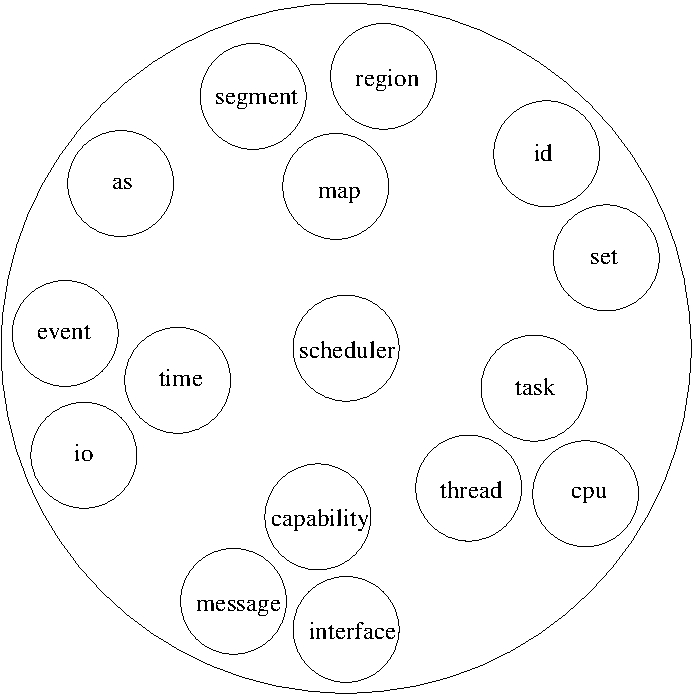
\includegraphics[scale=0.7]{\path/figures/managers-organisation.pdf}
    \caption{kaneton managers.}
    \label{figure:managers-organisation}
  \end{center}
\end{figure}

Note that this decomposition has no direct relation with the \textit{Object
Programming} paradigm. Indeed, even if kaneton designers tried to reduce the
dependencies between the managers, some managers remain intrusive as they
access the data structures of one or more other managers.

A kaneton object represents a kernel entity. Every object is identified by
a \textbf{kaneton identifier} and protected by a \textbf{kaneton capability}
over the operating and distributed system.

Below are listed the most important objects:

\begin{itemize}
  \item
    A \textbf{segment} represents a continuous area of physical memory.
  \item
    A \textbf{region} represents a continuous area of virtual memory which
    maps a part of or a whole \textit{segment}.
  \item
    An \textbf{as} or \textbf{address space} represents a set of physical
    memory areas which can potentially be accessed through a set of virtual
    memory addresses.

    \-

    An \textit{as} is composed of a set of \textit{segments} and a set of
    \textit{regions}.
  \item
    A \textbf{task} represents a complete execution context.

    \-

    However, a \textit{task} is not an active entity as it is not the
    one scheduled. Indeed, a \textit{task} is actually composed of an
    \textit{address space} and one or more \textit{threads}.
  \item
    A \textbf{thread} represents the active execution context in a
    \textit{task}.
  \item
    An \textbf{event} describes an external event including hardware
    events like interrupts as well as software events also known as
    \textit{system calls} or \textit{syscalls}.
  \item
    \textbf{Message}s are used for communicating betweens tasks.
\end{itemize}

The reader should notice that there is a hierarchical relation between
these objects as it is illustrated by \textit{Figure
\ref{figure:objects-hierarchy}}.

\begin{figure}[h]
  \begin{center}
    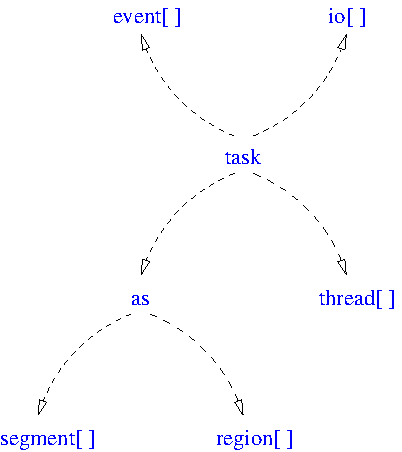
\includegraphics[scale=0.7]{\path/figures/objects-hierarchy.pdf}
    \caption{kaneton objects hierarchy.}
    \label{figure:objects-hierarchy}
  \end{center}
\end{figure}

XXX

overview: kernel = arch + generic :: data-struct + proc
expliquer ca dans overview pour introduire les sets!

XXX

There is another kaneton object which is internally widely used: the
\textbf{set} object. A \textit{set} object is an abstract data structure
managed by a dedicated manager, the \textit{set manager}. The \textit{set
manager} is used by the other kaneton managers for storing data without taking
care of how it is technically done. The set concept was introduced to make the
microkernel code as clear as pseudo code. For more information on the
\textit{set manager}, please refer to the book \textit{The kaneton
microkernel :: core}.

The kaneton microkernel was designed to be ported on many different - existing
or not - architectures. Therefore, the microkernel is divided into two
major components: the \textbf{core} and the \textbf{machine}. The \textit{core}
designs the kaneton source code which is independent from the underlying
computer. For more information on the \textit{core} component, please refer
to the appopriate book \textit{The kaneton microkernel :: core}. On the
contrary, the \textit{machine} component contains the source code related to
the underlying specific hardware.

Since a microprocessor architecture can be used on different mother boards
with various chipsets, the \textit{machine} component is also divided into
a \textbf{platform} which represents the board package; and a
\textbf{architecture} which represents the microprocessor.

Note that the behaviour of the \textit{machine} component can change depending
on the \textit{platform}/\textit{architecture} coupling. Therefore, the
\textbf{glue} was introduced to deal with the multiple
\textit{platform}/\textit{architecture} combinations.

\textit{Figure XXX} illustrates this decomposition. For more information on
the portability system, please refer to the \textit{Chapter
\ref{chapter:portability}}.

XXX [figure]

The kaneton microkernel provides powerful features for distributing computing
including security through capabilities but also communication through a
complete message passing system. Additionally, the microkernel already
integrates the notion of communicating node. As such, the microkernel knows
that the \textbf{distributed system} is composed of
  \textbf{machines}\footnote{The term \textit{machine} is used to represents
                             both the architecture-dependent microkernel's
                             source code and a computer in the distributed
                             system.},
each machine running a kaneton microkernel-based operating system. Moreover,
the communicating \textit{tasks} are named \textbf{nodes} in the distributed
system context.

\textit{Figure XXX} illustrates a distributed system composed of \textit{five}
machines and multiple \textit{nodes} which communicate with each other.

XXX [figure]

The kaneton microkernel is not directly launched when the computer is
turned on. Indeed, a \textbf{bootloader} first set up an execution environment
so that the kernel can be launched properly. The \textit{bootloader} takes
some \textbf{inputs} which represents additional files: configuration
files, execution files etc. For example, the first \textit{input} the
\textit{bootloader} uses is the kaneton microkernel binary file which is
loaded and launched by the \textit{bootloader} itself.

The kaneton microkernel manages tasks which are classified into \textit{four}
categories according to the privileges they get on the system. These different
classes of task are described next.

A \textbf{program} is the lowest priviliged task of the system. The common
user programs are the well known UNIX{\copyright} binaries like
\textit{/bin/ls}, \textit{/bin/sh} etc. A \textbf{service} is a microkernel
server which provides a logical service. For example, a service could be the
\textit{Virtual File System} which dispatches the calls to the file systems
servers. A \textbf{driver} is a service which performs hardware communication.
For example, a \textit{Wireless driver} is a \textit{driver} in the kaneton
terms. Finally, a \textbf{kernel} is a task which is a kind of super-driver
in which it has full rights on the whole underlying hardware.

For more information on the design on the kaneton microkernel, please
refer to the paper \textit{The kaneton microkernel project}.

%
% implementation
%

\section{Implementation}

This section focuses on the terminology used in the \textit{kaneton microkernel
research project} implementation. Obviously, this terminology is also used
in the educational project's context.

As explained in the previous section, the kaneton microkernel is subdivided
into multiples managers.

Each manager provides an interface to manipulate the kaneton object or
something the manager is in charge. The naming scheme used for these provided
functions is detailed below.

Recall that the interface provided by the set of kaneton managers is not
absolutely identical to the system call interface. Indeed, some functions
are private to the microkernel. Moreover, some functions of a manager's
interface must only be called by the manager itself and should not be called
by the other managers.

The couple of functions \textbf{initialize}() and \textbf{clean}() initialize
and clean the manager, respectively.

The function \textbf{show}() displays information on a given identified object
while the function \textbf{dump}() displays information on every objects
hold by the manager.

The function \textbf{reserve}() reserves an object given some properties. On
the contrary, the function \textbf{release}() releases it.

The function \textbf{clone}() clones an object. It is important to understand
that cloning an object does not just mean generating an identical object.
Indeed, cloning an object implies cloning every object this object holds or
depends on.

The function \textbf{give}() gives an object to another entity. The function
\textbf{flush}() cleans every object previously reserved.

The function \textbf{get}() is used to retrieve a kaneton object given its
identifier. Note that this function is private to the manager.

In addition, the kaneton managers generally provide functions for modifying
a property of a given identified object. Moreover, every manager provides
a function \textbf{attribute}() which can be used to retrieve the state
of an object's property.

% %
% ---------- header -----------------------------------------------------------
%
% project       kaneton
%
% license       kaneton
%
% file          /Users/francois/k...iew/lecture/kernels/future/boot/boot.tex
%
% created       julien quintard   [fri oct 24 17:31:58 2008]
% updated          [mon jan 26 21:56:52 2009]
%

%
% ---------- setup ------------------------------------------------------------
%

%
% path
%

\def\path{../../../..}

%
% template
%

%
% ---------- header -----------------------------------------------------------
%
% project       kaneton
%
% license       kaneton
%
% file          /home/mycure/kaneton/view/template/lecture.tex
%
% created       julien quintard   [wed may 16 18:17:26 2007]
% updated       julien quintard   [sun may 18 23:23:40 2008]
%

%
% class
%

\documentclass[8pt]{beamer}

%
% packages
%

\usepackage{pgf,pgfarrows,pgfnodes,pgfautomata,pgfheaps,pgfshade}
\usepackage[T1]{fontenc}
\usepackage{colortbl}
\usepackage{times}
\usepackage{amsmath,amssymb}
\usepackage{graphics}
\usepackage{graphicx}
\usepackage{color}
\usepackage{xcolor}
\usepackage[english]{babel}
\usepackage{enumerate}
\usepackage[latin1]{inputenc}
\usepackage{verbatim}
\usepackage{aeguill}

%
% style
%

\usepackage{beamerthemesplit}
\setbeamercovered{dynamic}

%
% verbatim stuff
%

\definecolor{verbatimcolor}{rgb}{0.00,0.40,0.00}

\makeatletter

\renewcommand{\verbatim@font}
  {\ttfamily\footnotesize\selectfont}

\def\verbatim@processline{
  {\color{verbatimcolor}\the\verbatim@line}\par
}

\makeatother

%
% -
%

\renewcommand{\-}{\vspace{0.4cm}}

%
% date
%

\date{\today}

%
% logos
%

\pgfdeclareimage[interpolate=true,width=34pt,height=18pt]
                {epita}{\path/logo/epita}
\pgfdeclareimage[interpolate=true,width=49pt,height=18pt]
                {upmc}{\path/logo/upmc}
\pgfdeclareimage[interpolate=true,width=25pt,height=18pt]
                {lse}{\path/logo/lse}

\newcommand{\logos}
  {
    \pgfuseimage{epita}
  }

%
% institute
%

\institute
{
  \inst{1} kaneton microkernel project
}

%
% table of contents at the beginning of each section
%

\AtBeginSection[]
{
  \begin{frame}<beamer>
   \frametitle{Outline}
    \tableofcontents[current]
  \end{frame}
}

%
% table of contents at the beginning of each subsection
%

\AtBeginSubsection[]
{
  \begin{frame}<beamer>
   \frametitle{Outline}
    \tableofcontents[current,currentsubsection]
  \end{frame}
}


%
% title
%

\title{Boot}

%
% document
%

\begin{document}

%
% title frame
%

\begin{frame}
  \titlepage
\end{frame}

%
% outline frame
%

\begin{frame}
  \frametitle{Outline}

  \tableofcontents
\end{frame}

%
% ---------- text -------------------------------------------------------------
%

%
% introduction
%

\section{Introduction}

\begin{frame}
  \frametitle{Introduction}

  A machine will not start an operating system automagically. There are a few steps before a kernel starts.

  \-

  This process is called the bootstrap. It is very specific to the machine, each architecture has its own bootstrap method.

  \-

  Through the bootstrap, the machine will provide some basic features that will be used to load the kernel, or by the kernel itself to drive the machine.

\end{frame}

\section{Generalities}
\subsection{CPU startup}
% 1)

\begin{frame}
  \frametitle{CPU startup}

  The CPU contains several registers that defines its behaviour.

  \-

  \begin{itemize}
  \item Program Counter
  \item Status registers
  \item \ldots
  \end{itemize}

  \-

  These registers must have a known value on reset.

  \-

  The caches must be initialized, there musn't be any random valid entries there.

  \-

  These initializations are purely hardware, a reset pin on the CPU is used to trigger this mechanism.

\end{frame}

\subsection{Firmware}

\begin{frame}
  \frametitle{Firmware}

  The CPU initializes its PC to a constant address on a reset (Reset vector). There must be some binary code here so that the CPU can execute some consistant instructions.

  \-

  This code is platform specific and is not likely to change. It is therefore in general stored in ROM chips, or in Flash EEPROM chips.

\end{frame}       

\begin{frame}
  \frametitle{Firmware role}

  In general, the firmware has several purposes :
  
  \-

  \begin{itemize}
  \item Initializing some peripherials
  \item Installing some services to ease the task of the user programs
  \item Finding a user program to run
  \item Loading the user program on the boot device and running it
  \end{itemize}

\end{frame}

\begin{frame}
  \frametitle{Peripherial initialization}

  The peripherials have their own configuration registers. They must also be configured on reset. The firmware will then configure the devices it needs :

  \-

  \begin{itemize}
  \item Video card
  \item Keyboard controller
  \item Hard disk controller
  \item {<old school>Floppy disk controller</old school>}
  \item USB Host controller
  \item Network interface
  \item \ldots
  \end{itemize}

  \-

  Since the peripherials might be different from one platform to another, and since the same peripherials can be used in several different ways with a CPU, the firmware contains basic drivers. These are specific to these peripherials and to the way they are used in a specific machine. A firmware will in general belong to one specific platform and won't probably work on another without modifications.

\end{frame}

\begin{frame}
  \frametitle{Services installation}

  To ease the task of the user program, the drivers contained in the firmware will be made available to the user program, so that the user program can have a standard way to access the base peripherials of every platform.

  \-

  The firmware will setup the RAM and the CPU so that a user program can call generic subprograms that will handle basic hardware operations.

  \-

  This interface has to be specified for a given architecture, so that a program written for this architecture can run on all compatible platforms.

\end{frame}

\begin{frame}
  \frametitle{Examples :: Openboot}

  OpenBoot (or OpenFirmware) is the firmware embedded in all Sun's
  SPARC based stations.

  \-

  OpenBoot offers many services necessary to the
  bootup phase. For example:

  \begin{itemize}
  \item
    Device-tree exploration (\emph{sibling}, \emph{child},
    \emph{getprop}\ldots)
  \item
    Device I/O (\emph{open}, \emph{read}, \emph{write}\ldots)
  \item
    MMU operations (\emph{map\_phys}, \emph{unmap\_phys}, \emph{itlb\_load},
    \emph{dtlb\_load}\ldots)
  \item
    Environment (boot path, boot device, boot arguments\ldots)
  \item
    Time (\emph{milliseconds})
  \end{itemize}

  \-

  All these functionnalities make OpenBoot a tiny OS. In addition,
  OpenBoot is able to run bytecode scripts (in Forth language), to
  load ELF files from disk or network (TFTP) and to debug programs
  (disassembly, registers dump, calls trace\ldots).

\end{frame}

\begin{frame}
  \frametitle{OpenBoot service call}

  Calling OpenBoot is as simple as jumping to the so-called
  \emph{firmware entry-point} (given in register \%g7 at boot time)
  with a structure in first argument (register \%o0). This structure is
  as follow:

  \begin{itemize}
  \item
    A pointer to a string indicating the name of the function to call.
  \item
    The number of arguments \emph{N}
  \item
    The number of return values \emph{M}
  \item
    \emph{N} 64-bit arguments
  \item
    \emph{M} 64-bit slots for results
  \end{itemize}

\end{frame}

\begin{frame}
  \frametitle{Examples :: ARCS}

  ARCS is the firmware used in all SGI MIPS-based stations. ARCS has
  also been used on a few Pentium-based stations, in replacement of
  the traditional BIOS.

  \-

  ARCS offers:

  \begin{itemize}
  \item
    Device-tree functions (\emph{GetPeer}, \emph{GetChild},
    \emph{GetComponent}\ldots)
  \item
    Device I/O (\emph{open}, \emph{read}, \emph{write}\ldots)
  \item
    Filesystem supports, FAT and ISO9660 (\emph{mount}, \emph{open},
    \emph{read}\ldots)
  \item
    Environment variables
  \item
    Time (\emph{GetTime})
  \end{itemize}

  \-

  ARCS is also able to load ELF files, from disk or network.

\end{frame}

\begin{frame}
  \frametitle{ARCS System Parameter Block}

  The System Parameter Block (SPB) is a structure filled by ARCS before giving the 
  hand to the boot program. The block contains notably the Firmware Vector, which is 
  an array of function pointers. Calling ARCS is as simple as calling the wanted function 
  from this vector. 

\end{frame}


\begin{frame}
  \frametitle{Examples :: (U)EFI}

  EFI (Extensible Firmware Interface) is a firmware specification made by Intel, and used in Itanium (IA-64) platforms. Apple also uses EFI in their new generation of Intel IA-32 machines.

  \-

  EFI has been designed to replace the BIOS that was far too limited, especially for High-end server platforms.

  \-

  An EFI firmware is mainly written in C while the BIOSes were written in ASM, and it uses 32-bit code where a BIOS used 16-bit code.

\end{frame}

\begin{frame}
  \frametitle{(U)EFI}

  EFI is still not included in standard PCs since it would break the backwards compatibility, which is a huge advantage of this architecture, compared to all others.

  \-

  EFI is extensible, it is composed of modules that can be loaded, and user can easily add or remove modules. The EFI standard describes a protocol to share services between the modules.
  
  \-

  An EFI firmware provides some advanced runtime services to the operating system, such as time, environment, device drivers for video, disk, network, filesystems, \ldots that can be called through a simple C function call from the operating system.

  \-

  EFI also provides a boot manager, that allow to select the boot device and directly start an operating system (the bootloader in that case is an EFI module), and a shell that allows to perform some basic actions.

\end{frame}

\subsection{Bootloader}

\begin{frame}
  \frametitle{Goal of the bootloader}

  A kernel, in order to start, generally requires a specific setup of the machine.

  \-

  It cannot rely on the firmware for that.

  \-

  A specific small program called bootloader will prepare the CPU for the kernel, find and load the kernel, and finally transfer the execution to the kernel.

  \-

\end{frame}

\begin{frame}
  \frametitle{Loading the kernel}

  The first task of the bootloader is to locate the kernel image. There are several possibilities: the kernel might be stored as raw data on some special blocks of a disk, it can also be stored as a file, on a filesystem, it could even be available on the network, through a TFTP server. For that reason, bootloaders may need to have some filesystem drivers, or network interface drivers with a small IP stack.

  \-

  Once the kernel has been located, it must be loaded in memory. The kernel image can take several forms. It can be an ELF binary, it can be a Windows PE file, it can be a block of raw data to load at a specific address, it can be one of the previous compressed with gzip, \ldots The bootloader must know the file format of the kernel it loads.

  \-
  
  When the kernel is loaded, the bootloader must jump on its entry point. So the entry point must be specified, either as something constant, or through an address provided in the kernel image.

\end{frame}

\begin{frame}
  \frametitle{Providing system information to the kernel}

  To boot correctly, a kernel may need to get some information from the system or from the user:

  \begin{itemize}
  \item RAM size, boot device
  \item boot options (graphic mode, root partition \ldots)
  \item modules information
  \end{itemize}

  \-

  The bootloader can pass information through to ways:

  \begin{itemize}
  \item the microprocessor registers
  \item an info structure written in memory. Most often, the structure base address is stored in a register. In some specific cases, this structure can also be found with a magic number.
  \end{itemize}

\end{frame}

\begin{frame}
  \frametitle{Bootloader specificities}

  In general, each kernel has its own dedicated bootloader, for each architecture it supports. For example : Lilo for Linux on x86, Silo for Linux on Sparc, \ldots.

  \-

  Some attempts have been made to make a standard. Grub for instance proposes the Multi-Boot Loader format. So Grub can boot every kernel that complies with the Multi-Boot Loader standard, like Linux, and FreeBSD for example.

\end{frame}

\section{x86 specificities}
\subsection{CPU startup}

\begin{frame}
  \frametitle{x86 CPU startup}

  The x86 CPU reset configures the CPU in Real-mode (16 bits, no segmentation, no paging, no privileges). This has been made to keep the compatibility within all the Intel x86 processors family.

  \- 

  The Reset vector value is 0xFFFFFFF0. This physical address is initialized by the motherboard so that it contains a jump to the firmware entry point.

\end{frame}

\subsection{Firmware}

\begin{frame}
  \frametitle{The BIOS}

  The firmware, on x86 platforms, is called BIOS (Basic Input/Output System). It is stored on a non volatile memory, and mapped by the hardware into the physical address space.

  \-

  The BIOS is a very primitive firmware, since they tried to keep the compatibility with old machines, so it didn't evolve much for years.

  \-

  The BIOS will first call the Video card's own BIOS. On x86, video cards have their own firmware that consists in x86 executable code.

  \-

  After this, the BIOS will initialize several peripherials and setup interrupt handlers to provide services (called BIOS Calls), so the user program can use these peripherials without any specific driver, by putting parameters in some registers and triggering a software interrupt.

\end{frame}

\begin{frame}
  \frametitle{The BIOS calls}

  The BIOS offers services to the bootloader/operating system. It setups some routines through a software interrupt interface.

  \-

  Several interrupt handlers are installed by the BIOS, each one concerns a type of operation, such as video, disk, floppy, \ldots.

  \-

  The actual operation is specified through the AX register, and optional parameters are passed through the other general purpose registers.

  \-

  Since the BIOS is 16-bit code, these BIOS services can only be called when the CPU is running in Real-mode. Since all modern operating systems are now running in protected mode, they can't use these BIOS calls. The VM86 mode allows to run 16-bit tasks in protected mode and is sometimes used to call BIOS calls from the protected mode, but in general, the kernels have their own device drivers and communicate directly with all the peripherials. So the BIOS calls are not really helpful to the kernels, and they are in general only used in the early boot stage, by the bootloader, before it switches to protected mode.

\end{frame}

\subsection{Bootloader}

\begin{frame}
  \frametitle{Boot sector}

  The BIOS, on the ia32 architecture, provides a way to boot from several devices, such as floppy disks or hard disks.

  \-

  1st sector of the devices (1 sector = 512 bytes)

  \-

  The bootloader will install itself in this sector.

\end{frame}

\begin{frame}
  \frametitle{Multi-stage bootloader}

  512 bytes is very small.

  \-

  Boot sector code = stage1.

  \-

  stage2+ are stored somewhere else

  \-

  stage1 role is to load stage2 (stage2 can be much bigger)

  \-

  Grub : 3 stages

\end{frame}

\begin{frame}
  \frametitle{The Multiboot standard}

  The Multiboot standard specifies an interface between a boot loader and a operating system.

  \-

  It aims at unifying kernel boot procedures in order to easily allow multiple OSes to coexist on the same machine.

  \-

  Multiboot specifications impose :

  \begin{itemize}
  \item an OS image format (to know how to load it and how to jump on it)
  \item Machine state
  \item Boot information format (structure of data passed to the kernel)
  \end{itemize}

\end{frame}

\begin{frame}
  \frametitle{Multiboot header}
  kernel image must :

  \begin{itemize}
  \item be an ordinary 32-bit executable file in the standard format for that particular operating system
  \item contain an additional header called Multiboot header. The Multiboot header must be contained completely within the first 8192 bytes of the OS image, and must be longword (32-bit) aligned.
  \end{itemize}

  \begin{tabular}{|l|l|l|l|l|}
  \hline
  Offset & Type & Field & Description & NameNote\\\hline\hline
  0 & u32 & magic & multiboot magic & required\\\hline
  4 & u32 & flags & flags & required\\\hline
  8 & u32 & checksum & checksum & required\\\hline
  12 & u32 & header\_addr & multiboot header addr & if flags[16] is set\\\hline
  16 & u32 & load\_addr & .text physical addr & if flags[16] is set\\\hline
  20 & u32 & load\_end\_addr & .data end & if flags[16] is set\\\hline
  24 & u32 & bss\_end\_addr & .bss physical end & if flags[16] is set\\\hline
  28 & u32 & entry\_addr & entry point physical addr & if flags[16] is set\\\hline
  32 & u32 & mode\_type  & graphic mode & if flags[2] is set\\\hline
  36 & u32 & width & number of columns & if flags[2] is set\\\hline
  40 & u32 & height & number of lines & if flags[2] is set\\\hline
  44 & u32 & depth & depth & if flags[2] is set\\\hline
  \end{tabular}

\end{frame}

\section{Conclusion}
\begin{frame}
  \frametitle{Conclusion}

  There is no standard bootstrap, each architecture has its own standard, that provides a way of setting up the machine, and providing services to the kernel.

  \-

  A bootloader is always required to fill the hole between the machine firmware and the operating system kernel.

  \-

  A bootloader is a quite small piece of code, but it is mandatory. A kernel cannot start without a working bootloader.

  \-

  To avoid the need of writing a new bootloader each time people is making a new kernel, some standards have been setup, but they are still not used by all the main operating systems.

\end{frame}

%
% bibliography
%

\begin{frame}[allowframebreaks]
  \frametitle{Bibliography}

  \bibliographystyle{amsplain}
  \bibliography{\path/bibliography/bibliography}
\end{frame}

\end{document}

%
% ---------- header -----------------------------------------------------------
%
% project       kaneton
%
% license       kaneton
%
% file          /Users/francois/k...rnels/future/portability/portability.tex
%
% created       julien quintard   [fri oct 24 17:31:58 2008]
% updated          [mon jan 26 21:58:11 2009]
%

%
% ---------- setup ------------------------------------------------------------
%

%
% path
%

\def\path{../../../..}

%
% template
%

%
% ---------- header -----------------------------------------------------------
%
% project       kaneton
%
% license       kaneton
%
% file          /home/mycure/kaneton/view/template/lecture.tex
%
% created       julien quintard   [wed may 16 18:17:26 2007]
% updated       julien quintard   [sun may 18 23:23:40 2008]
%

%
% class
%

\documentclass[8pt]{beamer}

%
% packages
%

\usepackage{pgf,pgfarrows,pgfnodes,pgfautomata,pgfheaps,pgfshade}
\usepackage[T1]{fontenc}
\usepackage{colortbl}
\usepackage{times}
\usepackage{amsmath,amssymb}
\usepackage{graphics}
\usepackage{graphicx}
\usepackage{color}
\usepackage{xcolor}
\usepackage[english]{babel}
\usepackage{enumerate}
\usepackage[latin1]{inputenc}
\usepackage{verbatim}
\usepackage{aeguill}

%
% style
%

\usepackage{beamerthemesplit}
\setbeamercovered{dynamic}

%
% verbatim stuff
%

\definecolor{verbatimcolor}{rgb}{0.00,0.40,0.00}

\makeatletter

\renewcommand{\verbatim@font}
  {\ttfamily\footnotesize\selectfont}

\def\verbatim@processline{
  {\color{verbatimcolor}\the\verbatim@line}\par
}

\makeatother

%
% -
%

\renewcommand{\-}{\vspace{0.4cm}}

%
% date
%

\date{\today}

%
% logos
%

\pgfdeclareimage[interpolate=true,width=34pt,height=18pt]
                {epita}{\path/logo/epita}
\pgfdeclareimage[interpolate=true,width=49pt,height=18pt]
                {upmc}{\path/logo/upmc}
\pgfdeclareimage[interpolate=true,width=25pt,height=18pt]
                {lse}{\path/logo/lse}

\newcommand{\logos}
  {
    \pgfuseimage{epita}
  }

%
% institute
%

\institute
{
  \inst{1} kaneton microkernel project
}

%
% table of contents at the beginning of each section
%

\AtBeginSection[]
{
  \begin{frame}<beamer>
   \frametitle{Outline}
    \tableofcontents[current]
  \end{frame}
}

%
% table of contents at the beginning of each subsection
%

\AtBeginSubsection[]
{
  \begin{frame}<beamer>
   \frametitle{Outline}
    \tableofcontents[current,currentsubsection]
  \end{frame}
}


%
% title
%

\title{Portability}

%
% document
%

\begin{document}

%
% title frame
%

\begin{frame}
  \titlepage
\end{frame}

%
% outline frame
%

\begin{frame}
  \frametitle{Outline}

  \tableofcontents
\end{frame}

%
% ---------- text -------------------------------------------------------------
%

%
% introduction
%

\section{Introduction}

\begin{frame}
  \frametitle{Introduction}

  Nowadays, a lot of CPU types exist (IA-32, IA-32\_64, IA-64, ARM, ARM, MIPS, PowerPC, SH, m68k, Blackfin, ...) and a lot of machines uses these CPUs, in different ways.

  \-

  The modern operating systems are trying to cope with that, and they tend to support all these platforms, so that a user can use the same system on all the different machines he uses.

  \-

  Portability requires some design in the kernel, to avoid rewriting everything from scratch and maintaining a separate branch for each supported architecture.

  \-

  This course describes what are the differences between machines, and how to design a kernel so it can be ported on several platforms.

\end{frame}

\section{Architecture}
\subsection{Machine architecture vs CPU architecture}

\begin{frame}
  \frametitle{Machine architecture vs CPU architecture}

  From a kernel point of view, there are two kind of architectures on a machine :

  \begin{itemize}
  \item The CPU Architecture
  \item The Machine/Platform Architecture
  \end{itemize}

  \-

  The following slides will explain what makes a CPU architecture specific, what makes a Machine architecture specific, and how a kernel can be designed so it can be as easily as possible ported on several machines.  

\end{frame}

\subsection{Microprocessor architecture}

\begin{frame}
  \frametitle{Microprocessor architecture}

  The architecture of a microprocessor defines :

  \begin{itemize}
  \item Its intructions set
  \item Its registers
  \item Its operational modes/behaviour
  \end{itemize}

  \-

  It's the interface between the software and the CPU itself, so it's basically what will be documented by the manufacturer in the datasheet of the CPU.

\end{frame}

\begin{frame}
  \frametitle{Microprocessor architecture}
  
  Several microprocessors models can share the same architecture.

  \-

  IA32 (commonly called x86) processors are manufactured by Intel, AMD, Via, \ldots

  \-

  ARM designs CPU architectures, manufacturers can use these specifications to make their own CPU.

\end{frame}

\begin{frame}
  \frametitle{Microprocessor architecture extensions}

  Some manufacturers are expanding one CPU architecture to provide more features, but keeping the main CPU architecture as a base.

  \-

  A code that was made to run on the base architecture will work on all the derivatives architectures, but not the opposite.

  \-

  This approach has been used quite a lot, for example, with IA-32 architecture, and the additional instruction sets (MMX, SSE, SSE2, SSE3 from Intel, 3dNow from AMD)

  \-

  A portable kernel would use these features if they are available, but must provide a software alternative in the other case. That way, the kernel can benefit from the performance gain provided by these instructions set, but doesn't depend on their presence to work.

\end{frame}

\begin{frame}
  \frametitle{CPU Architecture classes}

  Some categories have been made to distinguish families of CPU architectures :

  \begin{itemize}
  \item RISC Architecture: Reduced Instruction Set Computer - This family of CPU architectures focus on providing a really basic and simple set of instructions, and they try to optimize each instruction as much as possible, so that even something quite complex, that will require several instructions, could be faster than on a CPU where one single instruction would have been used. Such an architecture contains generally a lot of registers, so that programs can work as much as possible on data stored in registers instead of doing several memory accesses.

  \item CISC Architecture: Complex Instruction Set Computer - This family of CPU architectures focus more on providing a consequent set of instructions, so that some usual operations, that could be done using several elementary operations, are available through a single instruction. For that reason, the instruction set of a CISC CPU contains quite a lot of operations. This kind of CPU actually quite often contains a RISC CPU and a Microcode that describes how to do each instruction.

  \end{itemize}

\end{frame}

\begin{frame}
  \frametitle{Microprocessor internal and external architecture}

  All this was about external architecture.

  \-

  There is another kind of Microprocessor architecture : the internal architecture.

  \-

  This is how the CPU is actually achieving the implementation of the interface required by the external architecture.

  \-

  This is the CPU manufacturers core business, it's what makes the difference between two CPUs that have the same external architecture, like Intel vs AMD, or Via on IA-32 processors, since it's what makes the difference in terms of performance, power consumption, \ldots

\end{frame}

\subsection{Machine architecture}

\begin{frame}
  \frametitle{Machine architecture}
  
  A microprocessor can't work alone. It has interfaces to communicate with other components : memory buses, peripherial buses, interrupts lines, \ldots

  \-

  This provides a way to connect the memory required by the microprocessor, and some peripherials that can be useful in a machine, such as time-sources/clocks, user interfaces, data storage, network interfaces, \ldots

  \-

  The firmware provided in a machine is also something specific to the machine architecture since it provides services to interface with the hardware to the operating system.

  \-

  All these things are external components that are connected to the CPU in a specific way. A machine architecture describes the set of components that are used, and how they are connected together.

\end{frame}

\begin{frame}
  \frametitle{Machine architecture}

  The IBM-PC architecture is the most known architecture that uses an IA-32 CPU, but there are actually some other. SGI, for instance, made a machine based on an IA-32 CPU, but that was different from the IBM-PC architecture (SGI 320) since it didn't have a BIOS, but a firmware based on their own ARCS firmware they used on their other MIPS machines.

  \-

  More recently, Apple released their own architecture based on IA-32, where they also don't use the BIOS, but instead provide a firmware called EFI.

  \-

  Some other CPU architectures are used in several different machine architectures. For example, the MIPS R5000 CPU was used in the SGI Indy architecture, and in the Sony Playstation 2 architecture. These two machines use the same CPU architecture but they are totally different. An OS written for the SGI Indy won't work on the Sony Playstation 2.

  \-

  Almost every single Windows mobile based smartphone is a different Machine architecture, although they all share the ARM CPU architecture.

\end{frame}

\section{Kernel splitting}
\subsection{Independant part}

\begin{frame}
  \frametitle{Independant part}

  The independant part of a kernel consists in all the code that will work on every machine.

  \-

  It basically consists of all the code handling the kernel's concepts. For example, a task is a high level concept that we can find in almost all kernels. A portable kernel will be able to manage tasks on all the architectures it supports. Some of the task management done by the kernel consists in the manipulation of structures describing the task in a generic way. All this code does not rely on machines specific features, the same code will run and work on all machines. This is an independant code.

  \-

  Of course, creating a task will certainly require some specific actions as well. The goal of a portable kernel will be to isolate as much as possible those parts of the code, and to put as much things as possible in the independant part, to avoid redundancy in the dependant part.

  \-

  No ASM code can be found in the independant part since ASM is by definition dependant of the CPU architecture.

\end{frame}

\subsection{Dependant part}

\begin{frame}
  \frametitle{Dependant part}

  The dependant part of a kernel contains all the code that is aimed to support a specific feature of a CPU, a machine, or a specific hardware.

  \-

  Writing entries in the MMU cache is something specific to the CPU. It's generally done using some assembly instructions that are different from one CPU architecture to another. That's why it's a code that depends on the CPU architecture.

  \-

  Setting up the platform to trigger an interrupt on a regular basis is something specific to the Machine architecture. In general, a machine contains a dedicated hardware, connected to a CPU interrupt line. That's why configuring it is done by some code that depends on the Machine architecture.

  \-

  These examples are not always true : if a CPU embeds its own clock source that can trigger an interrupt internally, then the code to configure it is not Machine architecture dependant, but it is CPU architecture dependant.

\end{frame}

\subsection{Board support package (BSP)}

\begin{frame}
  \frametitle{Dependant part}

  Some kernels, especially the kernels for embedded operating systems, introduced the Board Support Package (BSP) concept.
  
  \-

  For example, Windows CE, Microsoft's kernel for embedded systems, is working on 3 CPU architectures : IA-32, ARM9, SuperH, but it runs on a lot of devices with a lot of various hardware devices. Each device has its own machine architecture, and its own set of peripherials. For that reason, each platform requires some specific code to make the kernel to work on it.

\end{frame}


\section{Kaneton portability}

\begin{frame}
  \frametitle{Kaneton Portability}

  The Kaneton microkernel is designed to be portable. For that reason, the code is splitted in several sections :

  \begin{itemize}
  \item Core
  \item Machine
  \begin{itemize}
  \item Architecture
  \item Platform
  \item Glue
  \end{itemize}
  \end{itemize}

\end{frame}

\subsection{Core}

\begin{frame}
  \frametitle{Kaneton Core}

  In the Kaneton design, the machine independant code is called Core.

  \-

  This section of code contains all the kernel code which is not specific to a machine. It contains the high level functions and code that are used for all the kernel internal operations, such as :
  \begin{itemize}
  \item Allocate physical memory
  \item Allocate and map virtual memory
  \item Create a new task
  \item Send a message between two tasks
  \item \ldots
  \end{itemize}

  Most of these operations don't require to do any CPU specific operations, but some of them do. For example, mapping virtual memory to physical memory requires to configure the MMU through the caches, this is something different for each CPU. For that reason, every function in the Core module of Kaneton will make a call to a potential machine dependant code.

  \-
  
  This is achieved through a macro called machine\_call.

\end{frame}

\subsection{Machine}

\begin{frame}
  \frametitle{Kaneton Architecture}
  
  This section of the Kaneton code contains all the code specific to the CPU architecture.

  \-

  This is mainly the code that will require to use specific assembly calls (inline assembly) or the code that works on data structures imposed by the CPU.

\end{frame}

\begin{frame}
  \frametitle{Kaneton Platform}
  
  This section of the Kaneton code contains all the code specific to the machine architecture.

  \-

  This is the code that will handle some peripherials attached to the CPU in a specific architecture, and that are used by the kernel itself.

\end{frame}

\begin{frame}
  \frametitle{Kaneton Glue}

  In the Kaneton design, the independant code (Core) calls the dependant code.

  \-

  To make it possible, the dependant code must have a generic interface, so that the Core code doesn't contain specifically any call to a function specific to an architecture.

  \-

  In Kaneton, the independant code and the dependant code functions share exactly the same prototypes, so that the Core code can call the Machine code in a generic way.

  \-

  For that reason, a wrapper was required, to implement the correct interface, that would then call the Architecture and the Machine code accordingly. This is the role of Glue.

\end{frame}

\section{Conclusion}

\begin{frame}
  \frametitle{Conclusion}

  In order to make a portable kernel, one must well distinguish what code can be reused for every machine, and what code is specific to the machine he is working on.

  \-

  This problem has now been addressed in most of the modern operating systems kernels (Linux, BSD, Windows CE, \ldots) with more or less style, but it's generally much better when a kernel has been designed to be portable from the beginning.

  \-

  This portability is very important nowadays, since the hardware is evolving fast. Making a new kernel without thinking about portability is a bad strategy since it makes it dependant on the durability of the architecture it is being made for.

  
\end{frame}


%
% bibliography
%

\begin{frame}[allowframebreaks]
  \frametitle{Bibliography}

  \bibliographystyle{amsplain}
  \bibliography{\path/bibliography/bibliography}
\end{frame}

\end{document}

%
% ---------- header -----------------------------------------------------------
%
% project       kaneton
%
% license       kaneton
%
% file          /home/mycure/kaneton/view/book/kaneton/references.tex
%
% created       julien quintard   [tue jun 19 15:36:51 2007]
% updated       julien quintard   [sun dec 16 17:33:44 2007]
%

%
% ---------- references -------------------------------------------------------
%

\chapter{References}
\label{chapter:references}

This chapter contains a listing of the kaneton documents that readers might
be interested in as well.

\newpage

%
% ---------- text -------------------------------------------------------------
%

This document aimed at presenting the kaneton microkernel and its organisation.

The books listed below go further by describing more precisely a specific
component of the kaneton microkernel:

\begin{enumerate}
  \item
    \textbf{The kaneton microkernel :: core}

    \-

    That document focuses on the design and implementation of the kaneton
    microkernel core through the different managers;
  \item
    \textbf{The kaneton microkernel :: \textit{architecture}}

    \-

    Theses documents tackle the implementation of kaneton on the given
    \textit{architecture}. Additionally, these documents contain information
    on platforms coupled with this architecture.

    \-

    Thes documents can be found in two forms, either public or private. Indeed,
    these documents contain information students must not have access to.

    \-

    The architectures currently documented are listed below:

    \begin{itemize}
      \item
	\textbf{ia32}

	\-

	\textit{Platforms}: \textbf{ibm-pc}
    \end{itemize}
\end{enumerate}

%
% ---------- header -----------------------------------------------------------
%
% project       kaneton
%
% license       kaneton
%
% file          /home/mycure/kaneton/view/book/core/licenses.tex
%
% created       julien quintard   [tue may 12 18:35:31 2009]
% updated       julien quintard   [tue may 12 18:35:33 2009]
%

%
% ---------- licenses ---------------------------------------------------------
%

\chapter{Licenses}
\label{chapter:licenses}

In this chapter we will details the kaneton-related licenses.

\newpage

%
% ---------- text -------------------------------------------------------------
%

The kaneton project might be considered as an open-project since source
code is provided.

Nevertheless this is not the case as this project is used as material for
operating system courses.

Therefore, people implementing the kaneton microkernel should not
make their source code available. To avoid problems, especially students
cheating, kaneton people decided to use a kaneton-specific license
forbidding source code distribution.

The \name{kaneton license} is based on a more generic license, the
\name{pedagogical licence}.

The next sections will contain these licenses' descriptions.

%
% pedagogical license
%

\section{Pedagogical License}

\textbf{TERMS AND CONDITIONS FOR COPYING, DISTRIBUTION AND MODIFICATION}

\begin{enumerate}
  \item
    This License applies to any program or other work which contains a
    notice placed by the copyright holder saying it may be distributed
    under the terms of this License. The "Program", below, refers
    to any such program or work, and a "work based on the Program"
    means either the Program or any derivative work under copyright law:
    that is to say, a work containing the Program or a portion of it,
    either verbatim or with modifications and/or translated into another
    language. (Hereinafter, translation is included without limitation in
    the term "modification".) Each licensee is addressed as "you".
  \item
    You must not copy or distribute copies of the Program's source
    code, object code or executable form without explicit authorization
    from the maintainers.

    If you have this authorization, you must conspicuously and
    appropriately publish on each copy an appropriate copyright notice
    and disclaimer of warranty; keep intact all the notices that refer
    to this License and to the absence of any warranty; and give any
    other recipients of the Program a copy of this License along with
    the Program.
  \item
    You may modify your copy or copies of the Program or any portion of
    it, thus forming a work based on the Program, provided that you
    meet all of these conditions :

    \begin{enumerate}
      \item
	You must not publish your work without explicit authorization
	from the maintainers.
      \item
	You must send to the maintainers any work that in whole or in
	part contains or is derived from the Program or any part thereof.
      \item
	You must cause any work that you send, that in whole or in
	part contains or is derived from the Program or any part thereof,
	to be licensed as a whole under the terms of this License.
      \item
	You must cause the modified files to carry prominent notices
	stating that you changed the files and the date of any change.
      \item
	If the modified program normally reads commands interactively
	when run, you must cause it, when started running for such
	interactive use in the most ordinary way, to print or display an
	announcement including an appropriate copyright notice and a
	notice that there is no warranty (or else, saying that you
	provide a warranty) and telling the user how to view a copy
	of this License. (Exception: if the Program itself is interactive
	but does not normally print such an announcement, your work based
	on the Program is not required to print an announcement.)
    \end{enumerate}
  \item
    Access to the Program's source is granted if either:

    \begin{enumerate}
      \item
	You want to make the Program evolve
      \item
	You have pedagogical goals
    \end{enumerate}

    These requirements apply to the modified work as a whole. If
    identifiable sections of that work are not derived from the Program,
    and can be reasonably considered independent and separate works in
    themselves, then this License, and its terms, do not apply to those
    sections when you distribute them as separate works. But when you
    distribute the same sections as part of a whole which is a work based
    on the Program, the distribution of the whole must be on the terms of
    this License, whose permissions for other licensees extend to the
    entire whole, and thus to each and every part regardless of who wrote
    it.

    Thus, it is not the intent of this section to claim rights or contest
    your rights to work written entirely by you; rather, the intent is to
    exercise the right to control the distribution of derivative or
    collective works based on the Program.

    In addition, mere aggregation of another work not based on the Program
    with the Program (or with a work based on the Program) on a volume of
    a storage or distribution medium does not bring the other work under
    the scope of this License.
  \item
    You may not copy, modify, sublicense, or distribute the Program
    except as expressly provided under this License. Any attempt
    otherwise to copy, modify, sublicense or distribute the Program is
    void, and will automatically terminate your rights under this
    License. However, parties who have received copies, or rights,
    from you under this License will not have their licenses
    terminated so long as such parties remain in full compliance.
  \item
    You are not required to accept this License, since you have not
    signed it. However, nothing else grants you permission to modify
    or distribute the Program or its derivative works. These actions
    are prohibited by law if you do not accept this
    License. Therefore, by modifying or distributing the Program (or
    any work based on the Program), you indicate your acceptance of
    this License to do so, and all its terms and conditions for
    copying, distributing or modifying the Program or works based on
    it.
  \item
    Each time you redistribute the Program (or any work based on the
    Program), the recipient automatically receives a license from the
    original licensor to copy, distribute or modify the Program subject
    to these terms and conditions. You may not impose any further
    restrictions on the recipients' exercise of the rights granted
    herein. You are not responsible for enforcing compliance by third
    parties to this License.
  \item
    If the distribution and/or use of the Program is restricted in
    certain countries either by patents or by copyrighted interfaces,
    the original copyright holder who places the Program under this
    License may add an explicit geographical distribution limitation
    excluding those countries, so that distribution is permitted only
    in or among countries not thus excluded. In such case, this License
    incorporates the limitation as if written in the body of this
    License.
  \item
    We may publish revised and/or new versions of this License from
    time to time. It may evolve considering new contributors
    needs. Contact us if you have any request. Such new versions will
    be similar in spirit to the present version, but may differ in
    detail to address new problems or concerns.
  \item
    If you wish to incorporate parts of the Program into other free
    programs whose distribution conditions are different, write to the
    author to ask for permission, we sometimes make exceptions for this.
  \item
    THERE IS NO WARRANTY FOR THE PROGRAM, TO THE EXTENT PERMITTED BY
    APPLICABLE LAW. EXCEPT WHEN OTHERWISE STATED IN WRITING THE
    COPYRIGHT HOLDERS AND/OR OTHER PARTIES PROVIDE THE PROGRAM "AS IS"
    WITHOUT WARRANTY OF ANY KIND, EITHER EXPRESSED OR IMPLIED,
    INCLUDING, BUT NOT LIMITED TO, THE IMPLIED WARRANTIES OF
    MERCHANTABILITY AND FITNESS FOR A PARTICULAR PURPOSE. THE ENTIRE
    RISK AS TO THE QUALITY AND PERFORMANCE OF THE PROGRAM IS WITH
    YOU. SHOULD THE PROGRAM PROVE DEFECTIVE, YOU ASSUME THE COST OF
    ALL NECESSARY SERVICING, REPAIR OR CORRECTION.
  \item
    IN NO EVENT UNLESS REQUIRED BY APPLICABLE LAW OR AGREED TO IN
    WRITING WILL ANY COPYRIGHT HOLDER, OR ANY OTHER PARTY WHO MAY
    MODIFY AND/OR REDISTRIBUTE THE PROGRAM AS PERMITTED ABOVE, BE
    LIABLE TO YOU FOR DAMAGES, INCLUDING ANY GENERAL, SPECIAL,
    INCIDENTAL OR CONSEQUENTIAL DAMAGES ARISING OUT OF THE USE OR
    INABILITY TO USE THE PROGRAM (INCLUDING BUT NOT LIMITED TO LOSS OF
    DATA OR DATA BEING RENDERED INACCURATE OR LOSSES SUSTAINED BY YOU
    OR THIRD PARTIES OR A FAILURE OF THE PROGRAM TO OPERATE WITH ANY
    OTHER PROGRAMS), EVEN IF SUCH HOLDER OR OTHER PARTY HAS BEEN
    ADVISED OF THE POSSIBILITY OF SUCH DAMAGES.
\end{enumerate}

%
% kaneton license
%

\section{kaneton License}

\textbf{TERMS AND CONDITIONS FOR COPYING, DISTRIBUTION AND MODIFICATION}

\begin{enumerate}
  \item
    This licence is nothing more than a link to the pedagogical licence.
  \item
    Any program under the kaneton licence is in fact under the terms and
    conditions of the pedagogical licence.
\end{enumerate}


\end{document}

--

--

bouger les figures dans view/figures
XXX dans book::kaneton, archi supportees, core, glue, machdep system, syscall
    interface, dans book::core, un fichier par manager.

--

expliquer t_init dand book:kaneton et ensute l'implem dans arch:XXX
